\documentclass{beamer}

\usepackage[utf8]{inputenc}
%\usepackage[T1]{fontenc}
%\usepackage[latin1]{inputenc}

\usetheme{Warsaw}

\title[Signal segmentation]{Functionnal data analysis applied to neurology}
\author{Clément Bonvoisin, Pierre Ludmann}
\institute{CMLA (ENS Cachan), Cognac-G (Paris V)}
\date{09/04/2014}

\graphicspath{neuro-seg/}
\setbeamersize{text margin left=1.4cm}
\begin{document}
\setbeamertemplate{navigation symbols}{}
\setbeamertemplate{footline}[frame number]
%\addtobeamertemplate{footline}{\hfill\insertframenumber/\inserttotalframenumber}

\begin{frame}
\titlepage
\end{frame}

\begin{frame}
\frametitle{Plan}
  \tableofcontents[hideallsubsections]
\end{frame}

\AtBeginSection[]
{
  \begin{frame}
  \tableofcontents[currentsection, hideothersubsections]
  \end{frame} 
}

\section{Familiarisation avec le problème}
\subsection{Motivations}
\begin{frame}
	\frametitle{Pourquoi ce travail ?}
	\begin{itemize}
		\item[Cerveau] humain encore assez mal connu
		\item[Certains] troubles neurologiques sont donc difficiles à diagnostiquer, traîter, comprendre, ...
		\item[Utiliser] les outils mathématiques sur les données médicales pour aider le monde hospitalier à développer des traitements efficaces
		\item[Maladies] liées à la marche
	\end{itemize}	
\end{frame}

\subsection{Protocole expérimental}

\begin{frame}
	\frametitle{L'expérience et son acquisition}
	\begin{itemize}
		\item[Trajet] du patient : 
		\item environ 6 secondes à l'arrêt
		\item marche sur 10 mètres
		\item demi-tour
		\item marche sur 10 mètres

		\item[Capture] des signaux par des centrales inertielles : 
		\item on s'intéresse à ceux fixées à la ceinture et au pied droit
		\item accélérations et vitesses angulaires
		\item enregistrées à 20 Hz/100 Hz
		\item replacées dans le référentiel \mbox{(antéro-postérieure, medio-latérale, verticale)}
	\end{itemize}
\end{frame}

\begin{frame}
	\frametitle{Les capteurs}

		\hspace*{-1.3cm}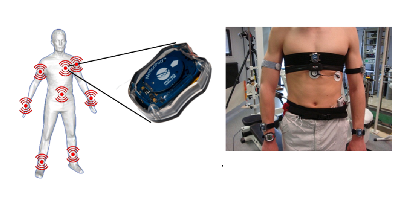
\includegraphics[scale=1.9]{capteurs.eps}

\end{frame}

\begin{frame}
	\frametitle{Exemple d'acquisition - Ceinture}

			\hspace*{-2.75cm}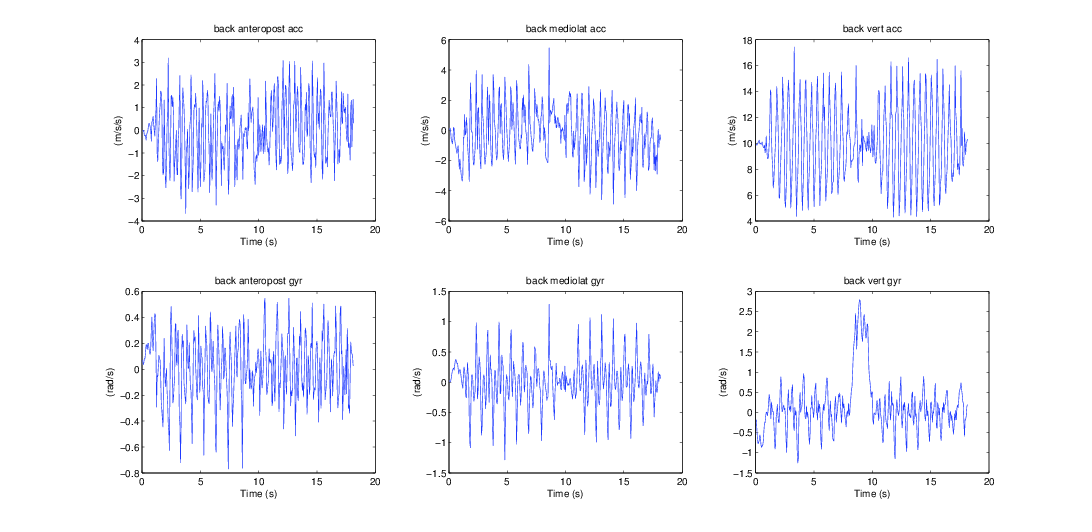
\includegraphics[scale=0.40]{examplevisuback}

\end{frame}

\begin{frame}
	\frametitle{Exemple d'acquisition - Pied}

			\hspace*{-2.75cm}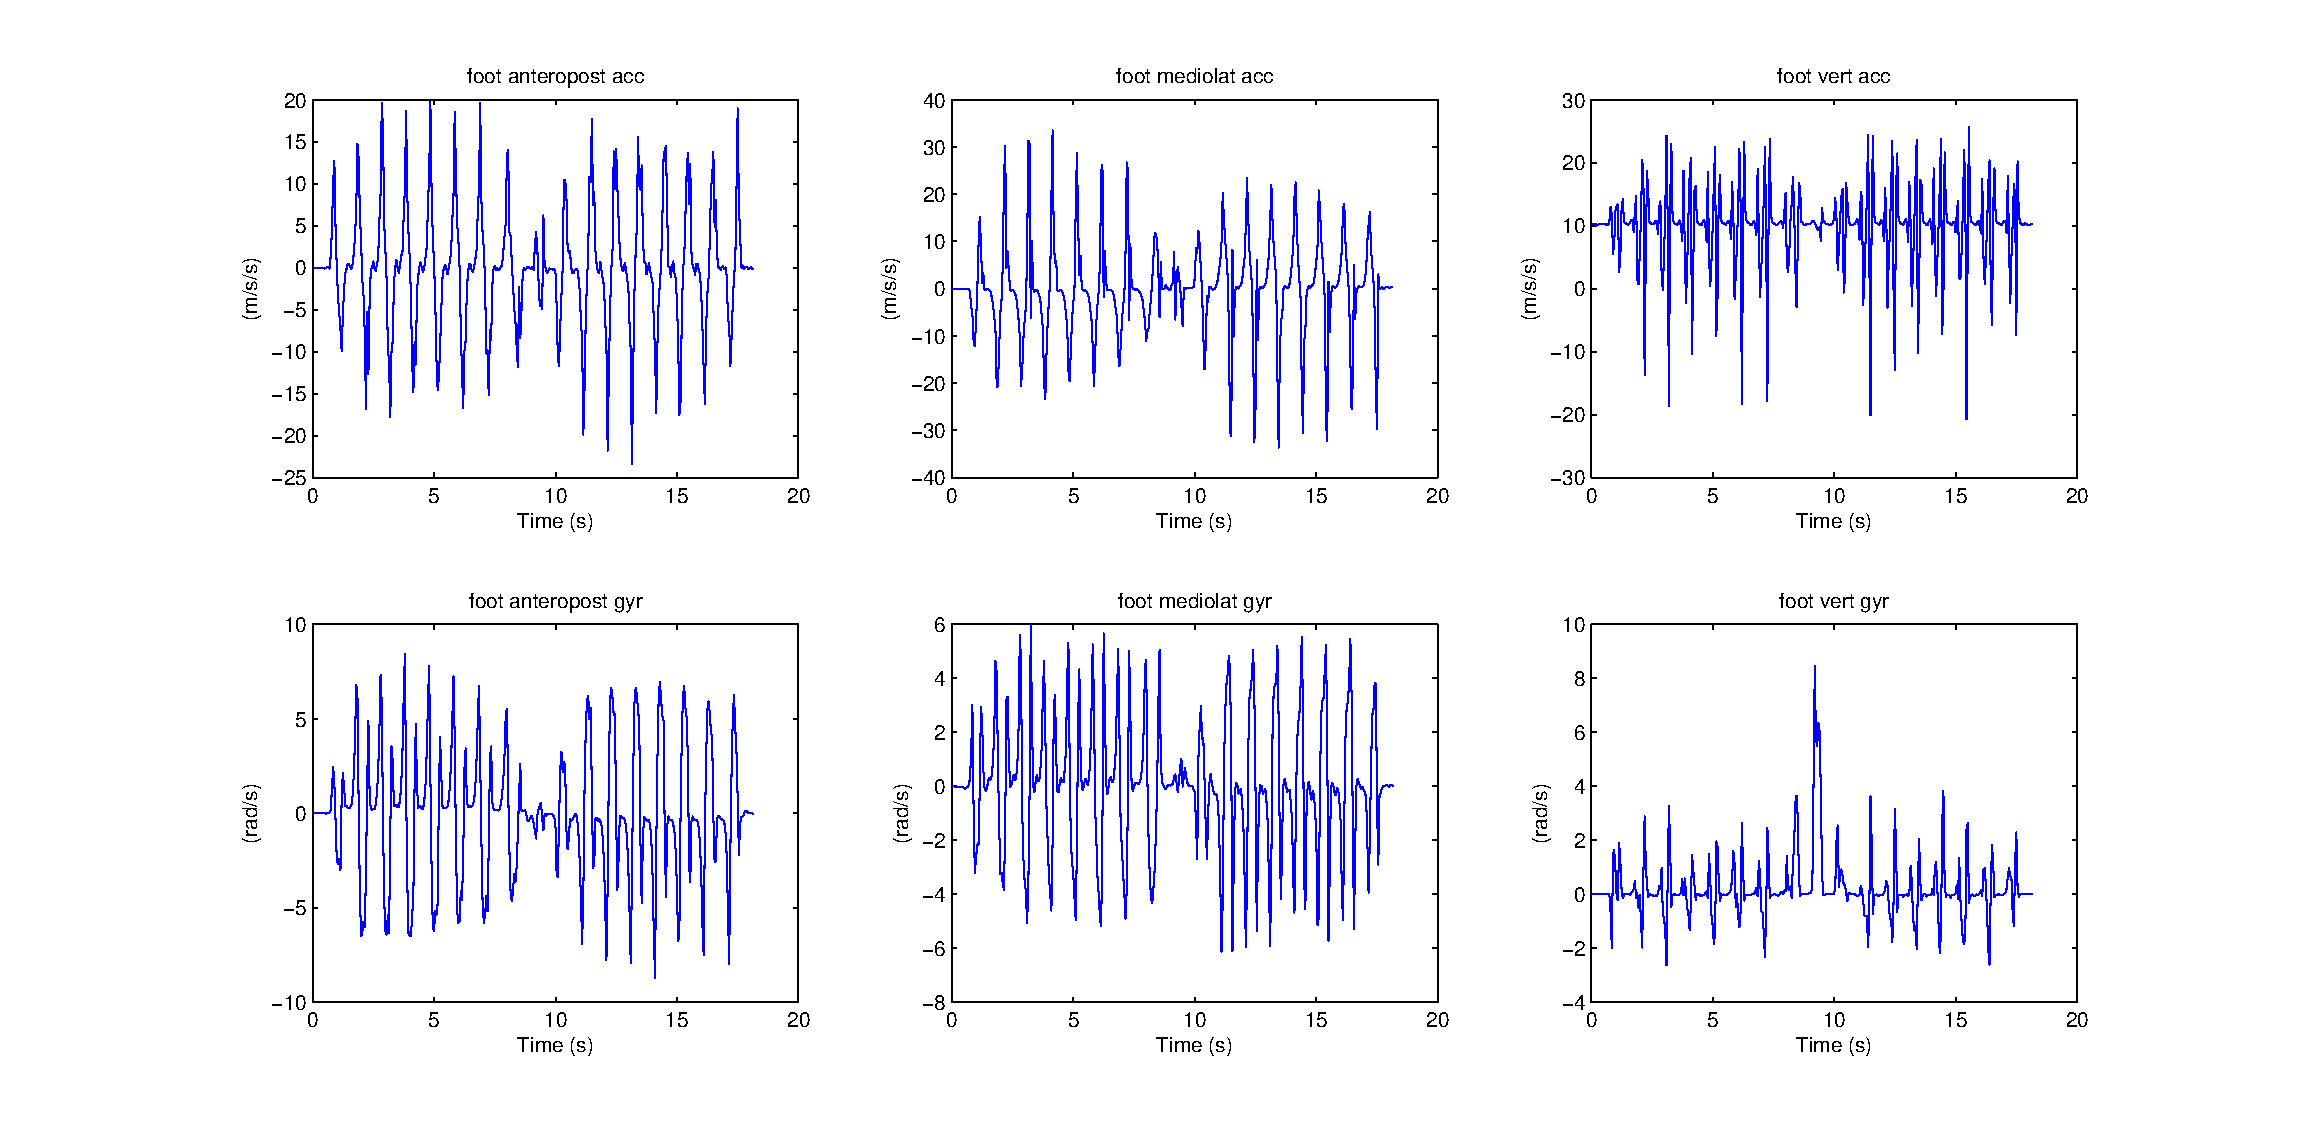
\includegraphics[scale=0.4]{examplevisufoot}

\end{frame}

\begin{frame}
	\frametitle{Exemple d'acquisition 2 - Ceinture}

			\hspace*{-2.75cm}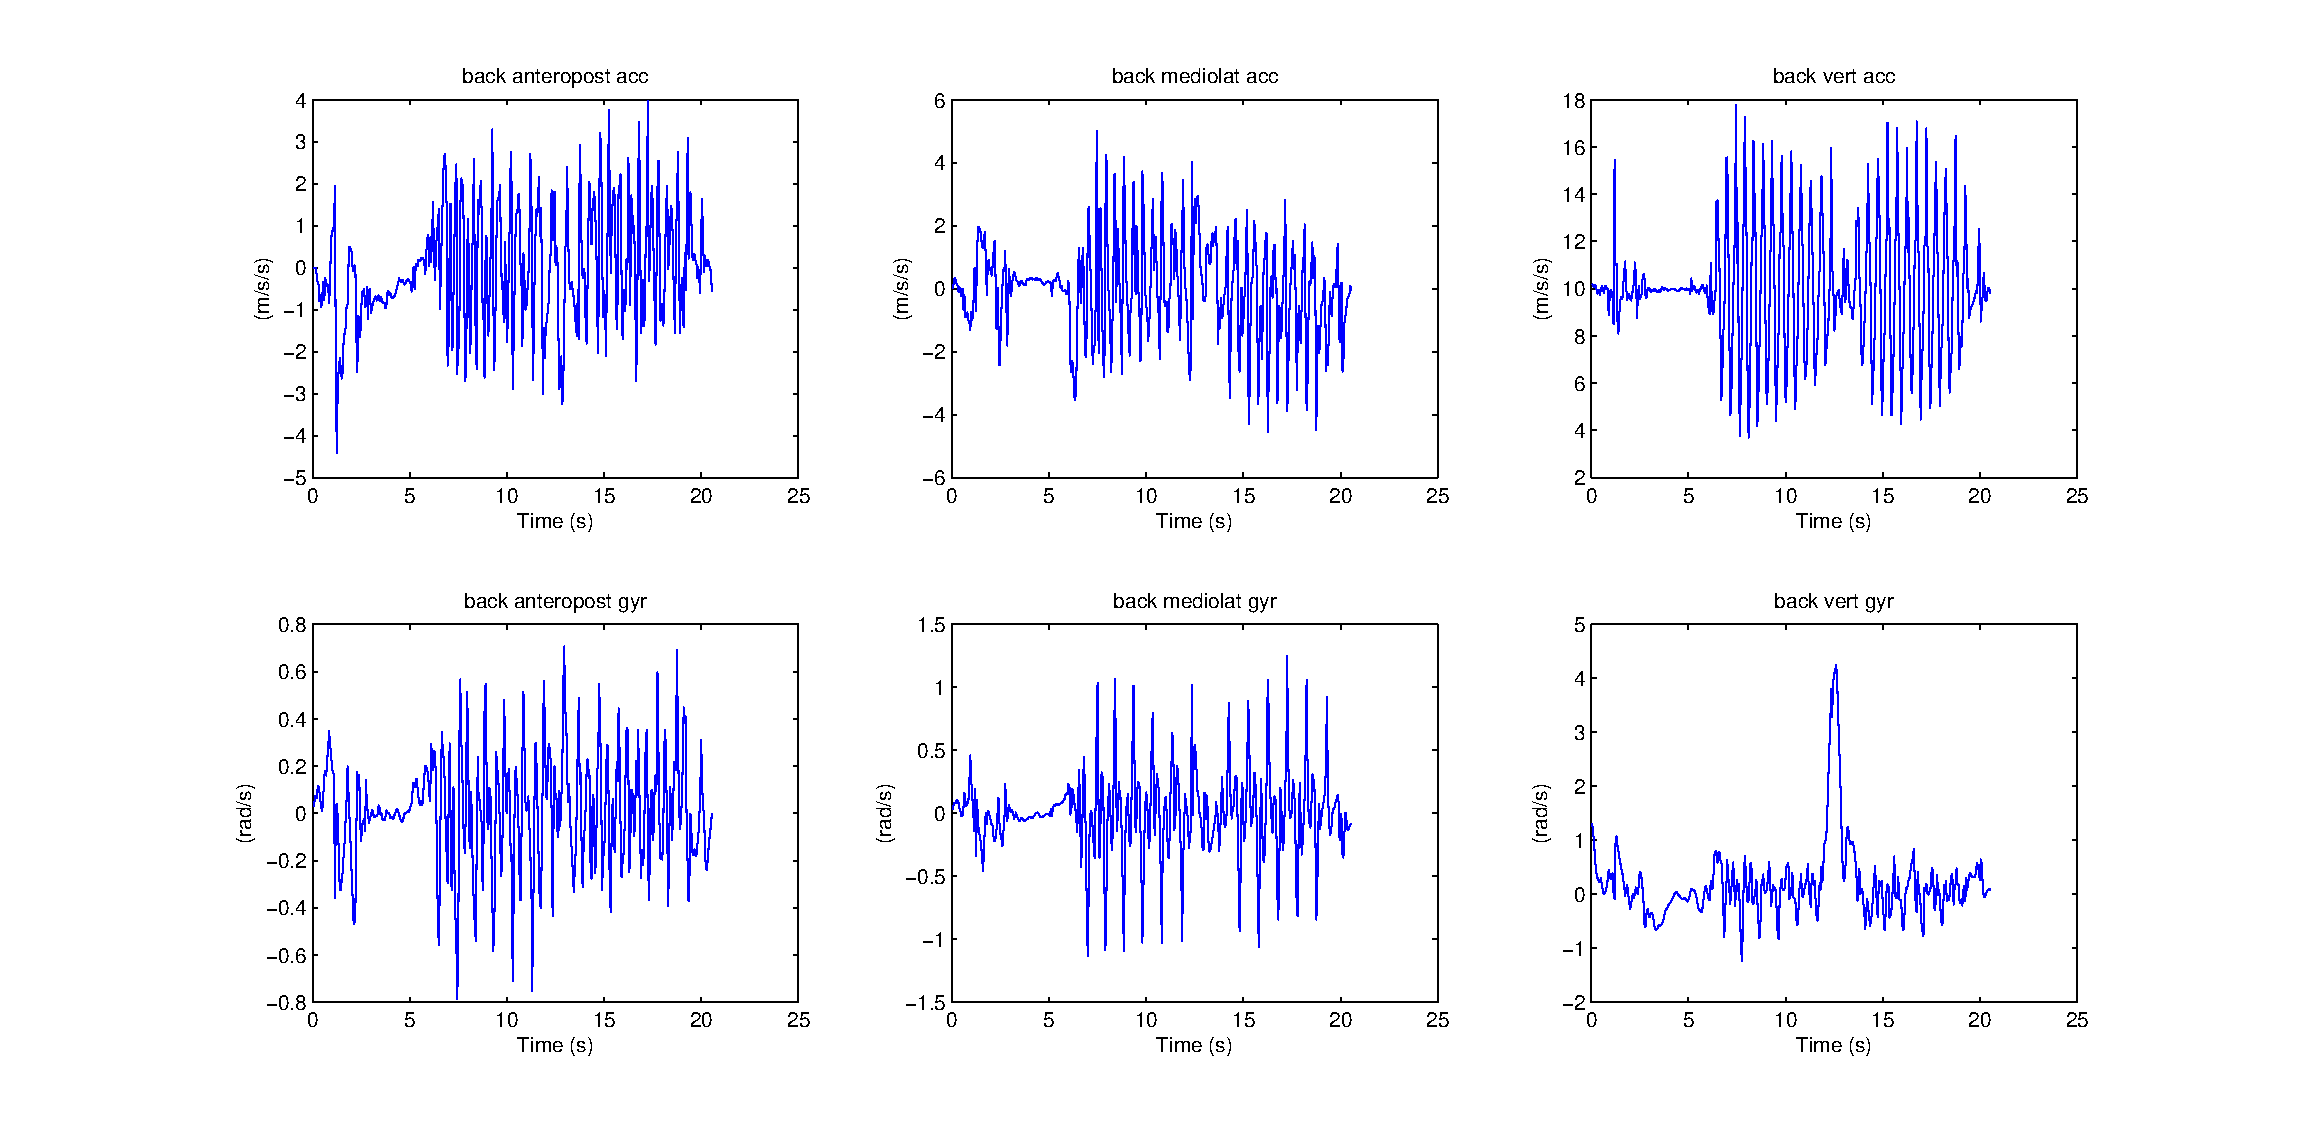
\includegraphics[scale=0.40]{errorexamplevisuback}

\end{frame}

\begin{frame}
	\frametitle{Exemple d'acquisition 2 - Pied}

			\hspace*{-2.75cm}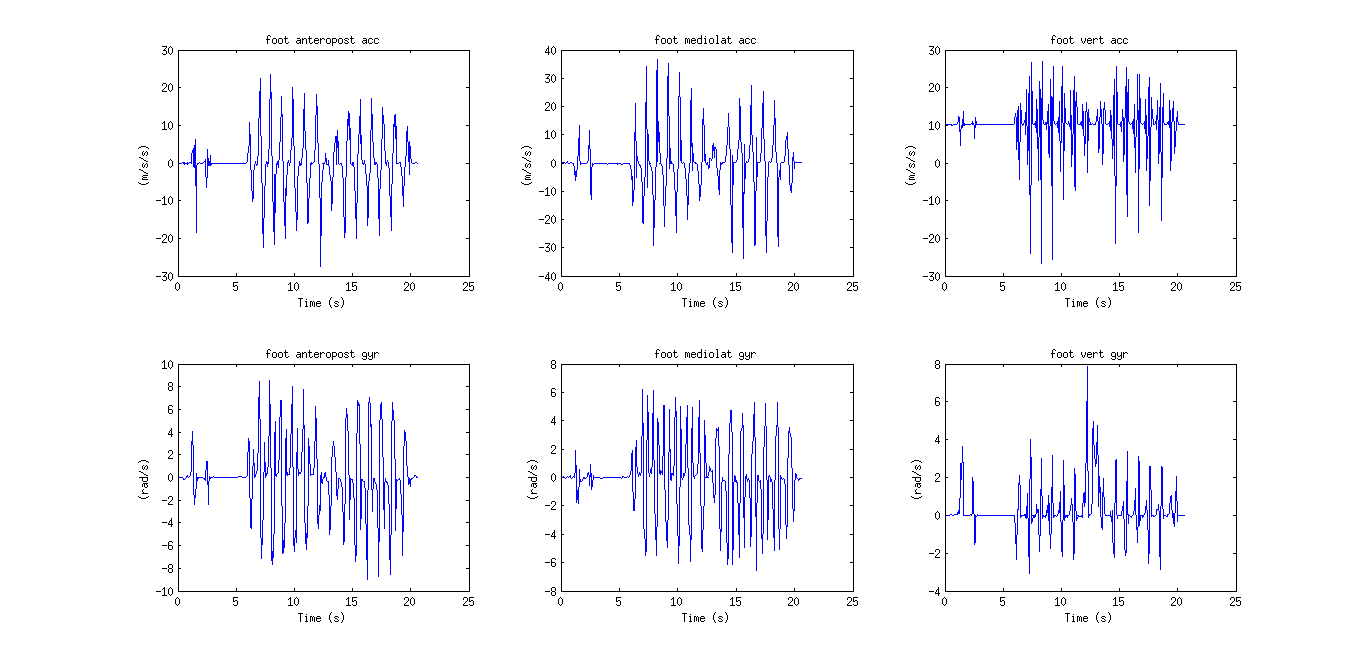
\includegraphics[scale=0.4]{errorexamplevisufoot}

\end{frame}
\subsection{Organisation du stage}

\begin{frame}
	\frametitle{Comment faire ?}
	\begin{itemize}
		\item[Signaux] sous extension .txt ou .csv
		\item[$\Longrightarrow$] Besoin de procédures pour importer au format .mat
		\vspace*{0.5cm}
		\item[D'abord] on segmente les signaux selon les différentes phases de l'expérience
		\item[Puis] on analyse les différents segments
		\vspace*{0.5cm}
		\item[L'affichage] montre clairement les différentes séquences de l'expérience
		\item[$\Longrightarrow$] La segmentation automatique doit être rapide et précise, au moins autant qu'à l'œil
	\end{itemize}
\end{frame}

\section{Segmentation des signaux}


\subsection{Algorithme CUSUM}

\begin{frame}
	\frametitle{Généralités sur l'algorithme CUSUM}
	\begin{itemize}
		\item[Biblio] \emph{Detection of Abrupt Changes : Theory and Application},\\
		M. Basseville, I. V. Nikiforov (1993)
		\item[Proposé] par E. S. Page dans \emph{Continuous inspection scheme} (1954)
		\item[Comparer] la meilleure hypothèse d'un changement de paramètre à la meilleure hypothèse stationnaire
		\item[Utilise] la vraisemblance logarithmique relative des hypothèses
	\end{itemize}
	\begin{equation}
		L _k =\ln \left[ \frac{\sup_{\theta_0}\prod_{i=1}^{k-1} p_{\theta_0}(y_i)\cdot\sup_{\theta_1}\prod_{i = k}^{N}p_{\theta_1}(y_i)}{\sup_{\tilde\theta}\prod_{i=i}^{N}p_{\tilde{\theta}}(y_i)} \right]
	\end{equation}
	\begin{itemize}
		\item[Rupture] au temps de vraisemblance maximale si dépasse un seuil
		\item[Complexité] élevée avec les bornes supérieures : besoin de simplification
	\end{itemize}
\end{frame}

\subsection{Hypothèses de travail}

\begin{frame}
	\frametitle{Le choix du gaussien}
	\begin{itemize}
		\item[Signaux] supposés suivre une distribution normale :
	\end{itemize}
	\begin{equation}
		p_{\mu, \sigma}(y) = \frac1{\sigma\sqrt{2 \pi}} \exp \left[ -\frac12 \left( \frac{y - \mu}{\sigma} \right)^2 \right]
	\end{equation}
	\begin{itemize}
		\item[Hypothèse] forte : indépendance temporelle et spatiale
		\item[Paramètre] $\theta$ : changement brusque de la moyenne et/ou de l'écart-type du signal
		\item[Hypothèse] utile : bornes supérieures atteintes aux estimateurs
	\end{itemize}
\end{frame}

\begin{frame}
	\frametitle{Choix des paramètres - Formules correspondantes}
	Trois choix possibles :
	\begin{itemize}
		\item[$\theta=\mu$]: on utilise (3) avec $\mu=\frac1n\sum_{i=1}^ny_i$ et $\sigma$ fixé
		\vspace*{.1cm}
		\item[$\theta=\sigma$]:  on utilise (4) avec $\mu$ fixé et $\sigma=\frac1n\sum_{i=1}^n(y_i-\mu)^2$
		\vspace*{.1cm}
		\item[$\theta=(\mu,\theta)$]: on utilise (4) avec $\mu=\frac1n\sum_{i=1}^ny_i$ et\\
		\hspace*{5.5cm}\mbox{$\sigma=\frac1n\left[\sum_{i=1}^ny_i^2-(\sum_{i=1}^ny_i)^2\right]$}
	\end{itemize}
	\vspace*{1cm}
	\begin{equation}
	\hspace{-1cm}	L_k=\frac 1{2\sigma^2}\left[(k-1)\mu_0^2+(N-k+1)\mu_1^2-N\tilde\mu^2\right]
	\end{equation}
	\begin{equation}
	\hspace{-1cm}	L_k=N\ln(\tilde\sigma)-(k-1)\ln(\sigma_0)-(N-k+1)\ln(\sigma_1)
	\end{equation}
\end{frame}




\subsection{Premiers résultats}

\begin{frame}
	\frametitle{Une segmentation}
	\hspace*{-2.8cm}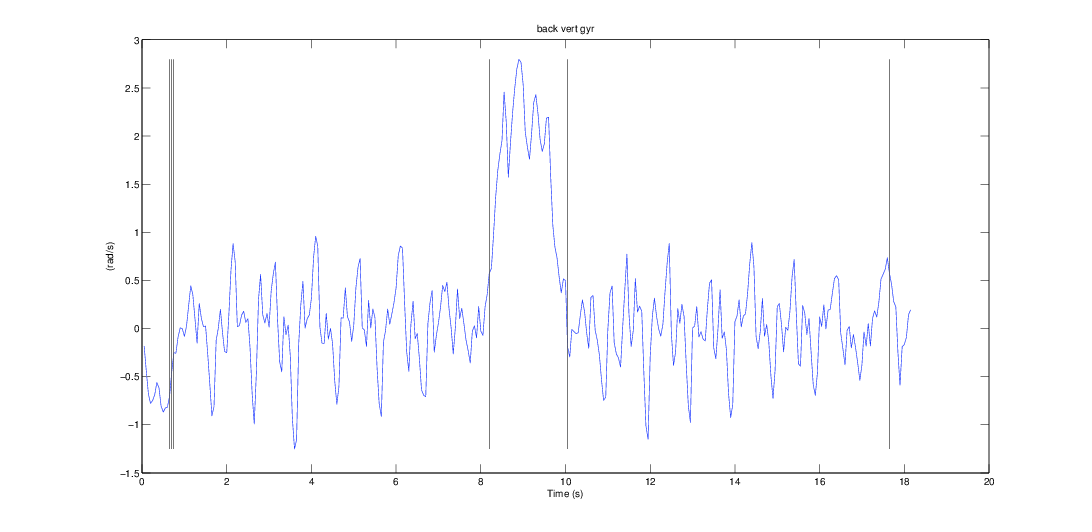
\includegraphics[scale=0.4]{examplecusumbackvertgyr}
\end{frame}

\begin{frame}
	\frametitle{Une segmentation}
	\hspace*{-2.8cm}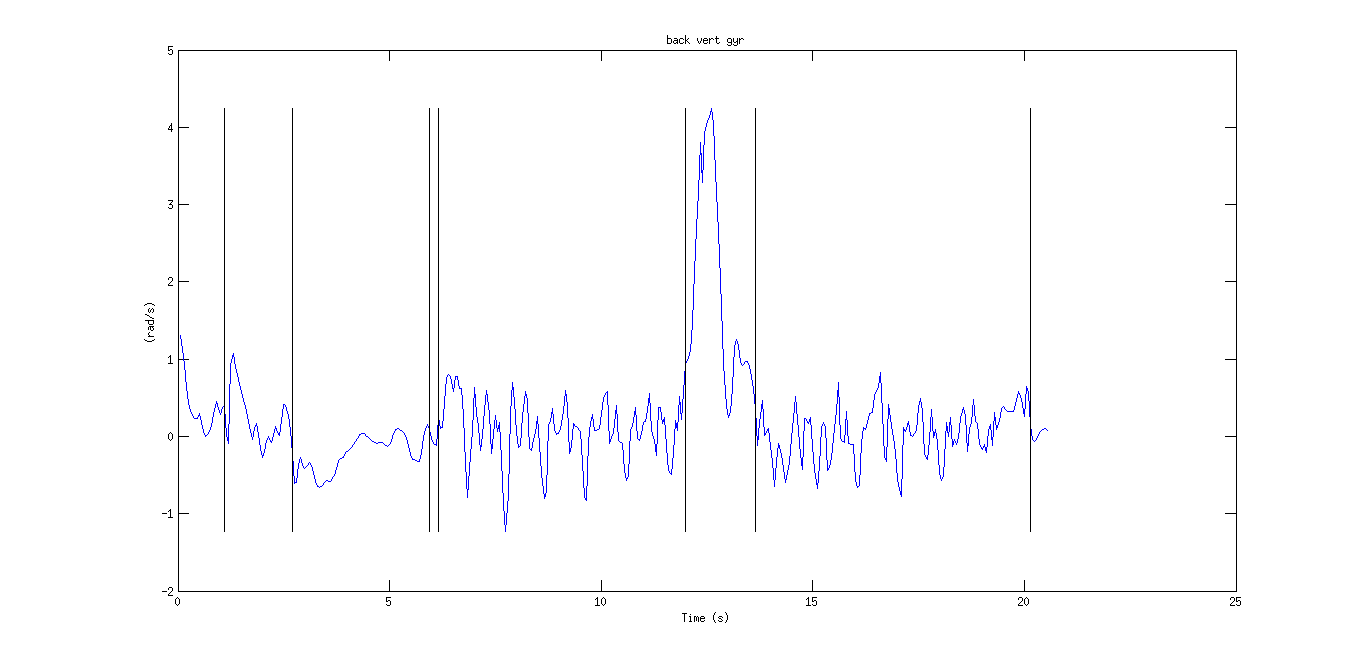
\includegraphics[scale=0.4]{errorexamplecusum}
\end{frame}

\section{Perspectives}

\begin{frame}
	\frametitle{Et maintenant ?}
	\begin{itemize}
		\item[Travail] sur les segments : différencier et détecter les différents types de maladies
		\item[$\Longrightarrow$] machine learning sur les segments obtenus
		\vspace*{1cm}
		\item[CUSUM] à généraliser sur des signaux quelconques
		\item[$\Longrightarrow$] adaptation du seuillage, des hypothèses
	\end{itemize}
\end{frame}

\end{document}